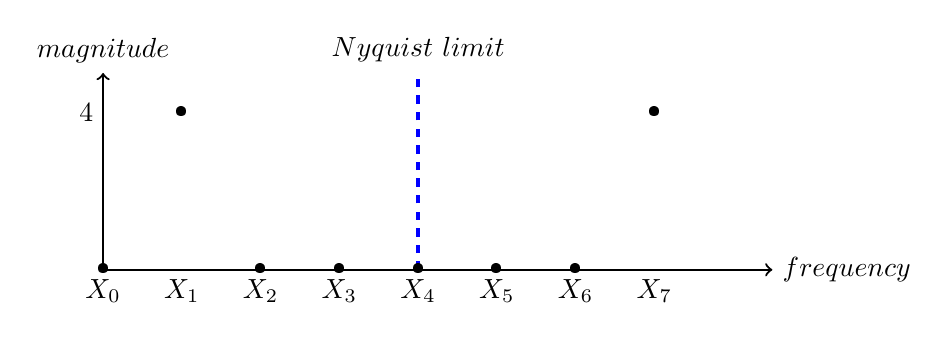
\begin{tikzpicture}
\draw[->,thick] (0,0)--(8.5,0) node[right]{$frequency$};
\draw[->,thick] (0,0)--(0,2.5) node[above]{$magnitude$};
\draw(0,2) node[left] {$4$};
\draw(0,0) node[below] {$X_0$};
\draw(1,0) node[below] {$X_1$};
\draw(2,0) node[below] {$X_2$};
\draw(3,0) node[below] {$X_3$};
\draw(4,0) node[below] {$X_4$};
\draw(5,0) node[below] {$X_5$};
\draw(6,0) node[below] {$X_6$};
\draw(7,0) node[below] {$X_7$};
\draw[ultra thick, blue, dashed] (4,0)--(4,2.5) node[black, above]{$Nyquist$ $limit$};
\foreach \Point in {(0,0),(1,2),(2,0),(3,0),(4,0),(5,0),(6,0),(7,2)}{
    \node at \Point {\textbullet};
}
\end{tikzpicture}